% !TEX root = ../SYSprojektrapport.tex
% SKAL STÅ I TOPPEN AF ALLE FILER FOR AT MASTER-filen KOMPILERES 

\section{Case 3: Husstandsbatteriers evne til at kompensere for tab af produktion}
I dette afsnit præsenteres resultater for simuleringen af case 3 iht. beskrivelsen i afsnit \ref{SimCase3}. I alle fire tilstande er spændingsændringen ved Town5 busbar (rød linje) og Transmission central 60kV busbar (Grøn linje) samt frekvensændringen på Transmission central 60kV busbar (Grøn linje), præsenteret på hhv. spændingsgraf og frekvensgraf. Derudover er der lavet opsamling over spænding samt effektoverførelse andre relevante steder i systemet i tabel \ref{fig:C3Overview}. \\ \\

\textbf{Tilstand 1: Alle batterierne er frakoblet.}
\begin{figure}[H]
	\centering
	\begin{minipage}[b]{0.48\textwidth}
		\centering
		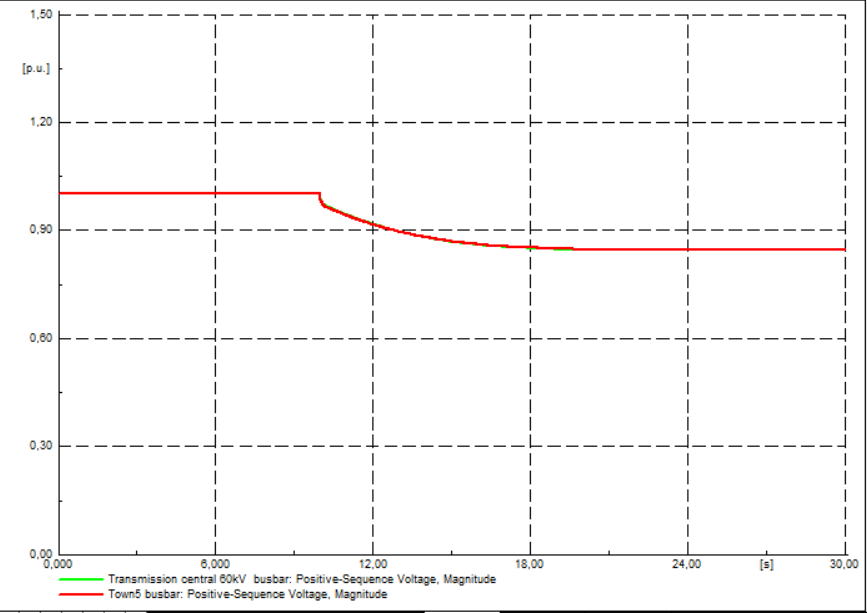
\includegraphics[width=1.00\textwidth]{figurer/LargeDisturbance/Voltage1} % Venstre billede
	\end{minipage}
	\hfill
	\begin{minipage}[b]{0.48\textwidth}
		\centering
		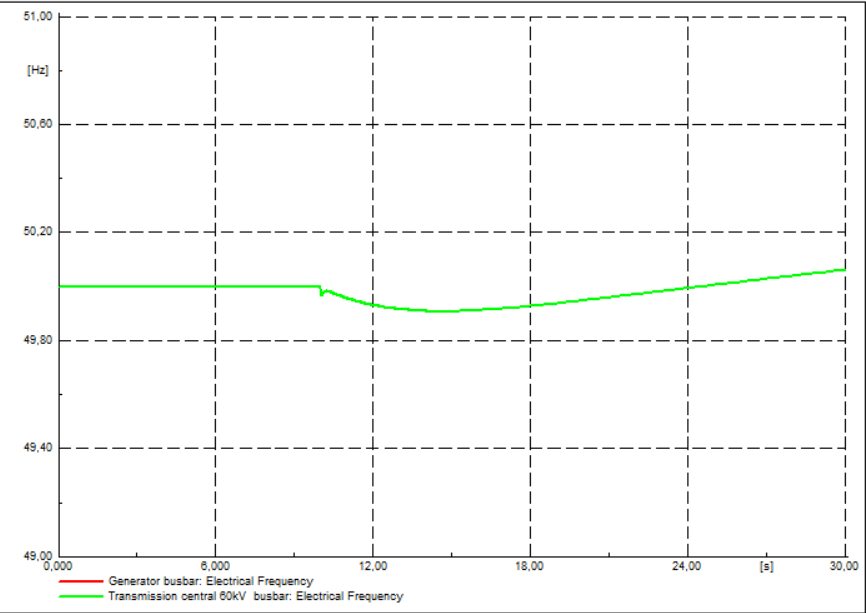
\includegraphics[width=1.00\textwidth]{figurer/LargeDisturbance/Freq1} % Højre billede
	\end{minipage}
	\\ % Figurtekster og labels
	\begin{minipage}[t]{0.48\textwidth}
		\caption{Case 2, Tilstand 1, Spændingsgraf} % Venstre figurtekst og label
		\label{fig:C2T1V}
	\end{minipage}
	\hfill
	\begin{minipage}[t]{0.48\textwidth}
		\caption{Case 2, Tilstand 1, Frekvensgraf} % Højre figurtekst og label
		\label{fig:C2T1F}
	\end{minipage}
\end{figure}

\textbf{Tilstand 2: Alle batterier leverer 0,5MW med pf 0,95 lagging.}
\begin{figure}[H]
	\centering
	\begin{minipage}[b]{0.48\textwidth}
		\centering
		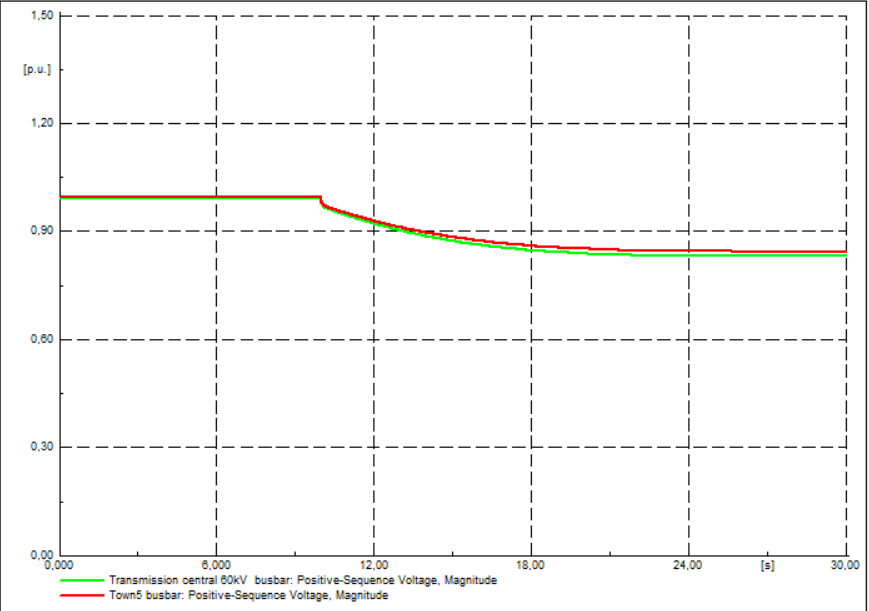
\includegraphics[width=1.00\textwidth]{figurer/LargeDisturbance/Voltage2} % Venstre billede
	\end{minipage}
	\hfill
	\begin{minipage}[b]{0.48\textwidth}
		\centering
		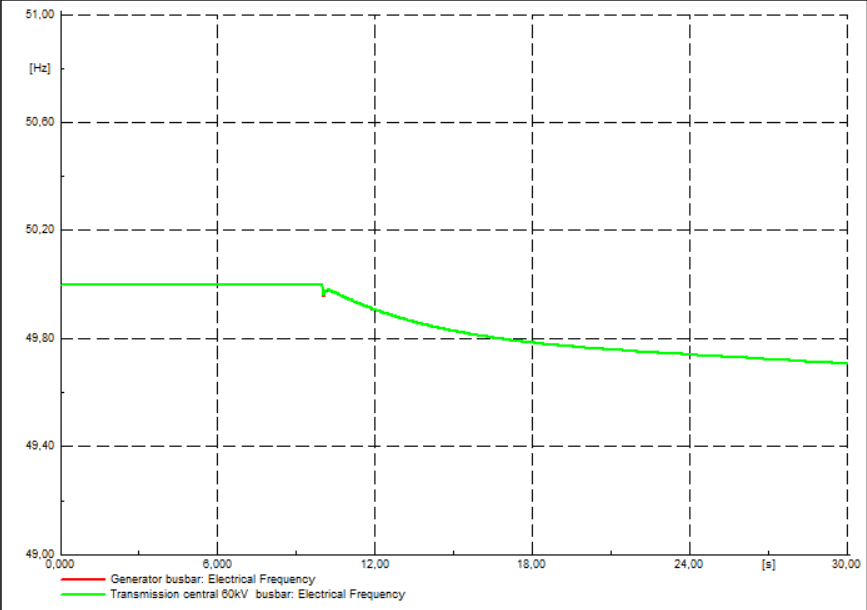
\includegraphics[width=1.00\textwidth]{figurer/LargeDisturbance/Freq2} % Højre billede
	\end{minipage}
	\\ % Figurtekster og labels
	\begin{minipage}[t]{0.48\textwidth}
		\caption{Case 2, Tilstand 2, Spændingsgraf} % Venstre figurtekst og label
		\label{fig:C2T2V}
	\end{minipage}
	\hfill
	\begin{minipage}[t]{0.48\textwidth}
		\caption{Case 2, Tilstand 2, Frekvensgraf} % Højre figurtekst og label
		\label{fig:C2T2F}
	\end{minipage}
\end{figure}

\textbf{Tilstand 3: Alle batterier leverer 1MW med pf 0,95 lagging.}
\begin{figure}[H]
	\centering
	\begin{minipage}[b]{0.48\textwidth}
		\centering
		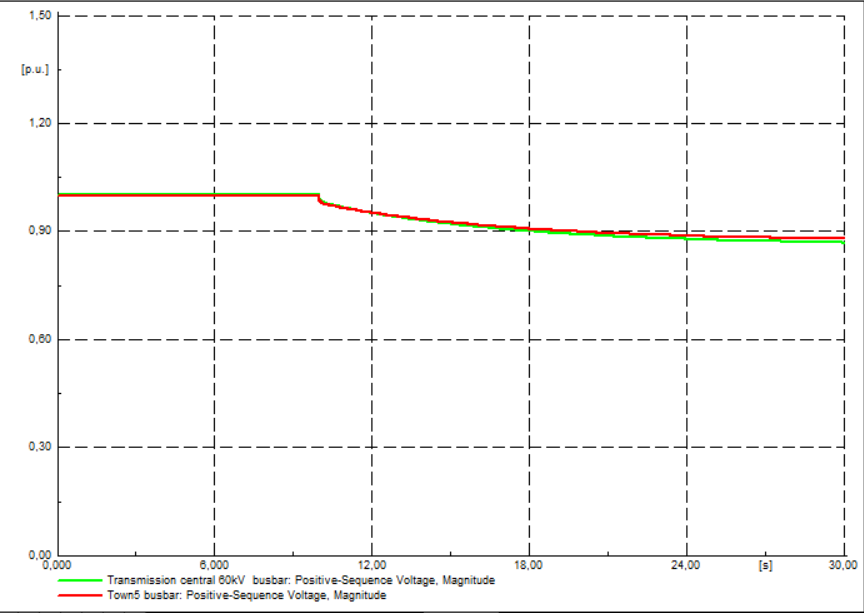
\includegraphics[width=1.00\textwidth]{figurer/LargeDisturbance/Voltage3} % Venstre billede
	\end{minipage}
	\hfill
	\begin{minipage}[b]{0.48\textwidth}
		\centering
		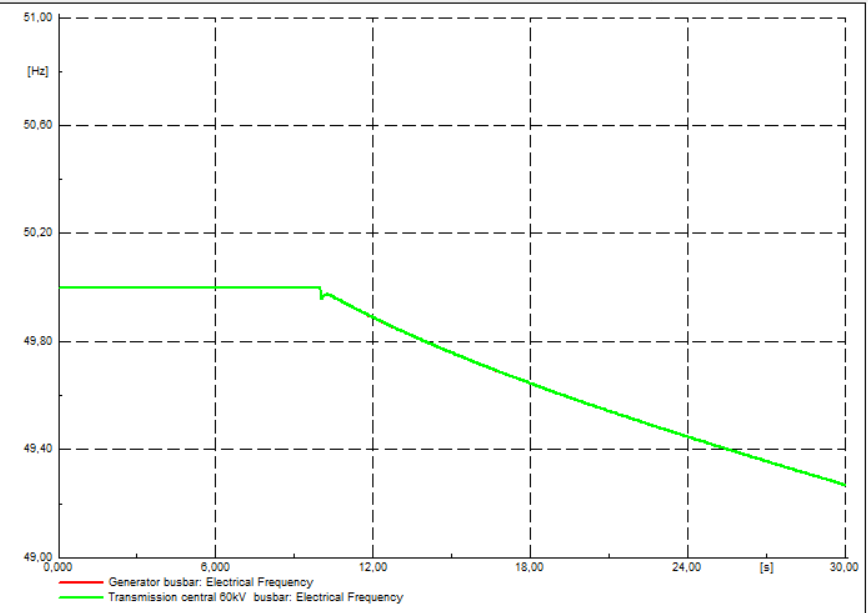
\includegraphics[width=1.00\textwidth]{figurer/LargeDisturbance/Freq3} % Højre billede
	\end{minipage}
	\\ % Figurtekster og labels
	\begin{minipage}[t]{0.48\textwidth}
		\caption{Case 2, Tilstand 3, Spændingsgraf} % Venstre figurtekst og label
		\label{fig:C2T3V}
	\end{minipage}
	\hfill
	\begin{minipage}[t]{0.48\textwidth}
		\caption{Case 2, Tilstand 3, Frekvensgraf} % Højre figurtekst og label
		\label{fig:C2T3F}
	\end{minipage}
\end{figure}

\textbf{Tilstand 4: Alle batterier leverer 1,35MW (Byerne kan betegnes som selvforsynende) med pf 0,95 lagging.}
\begin{figure}[H]
	\centering
	\begin{minipage}[b]{0.48\textwidth}
		\centering
		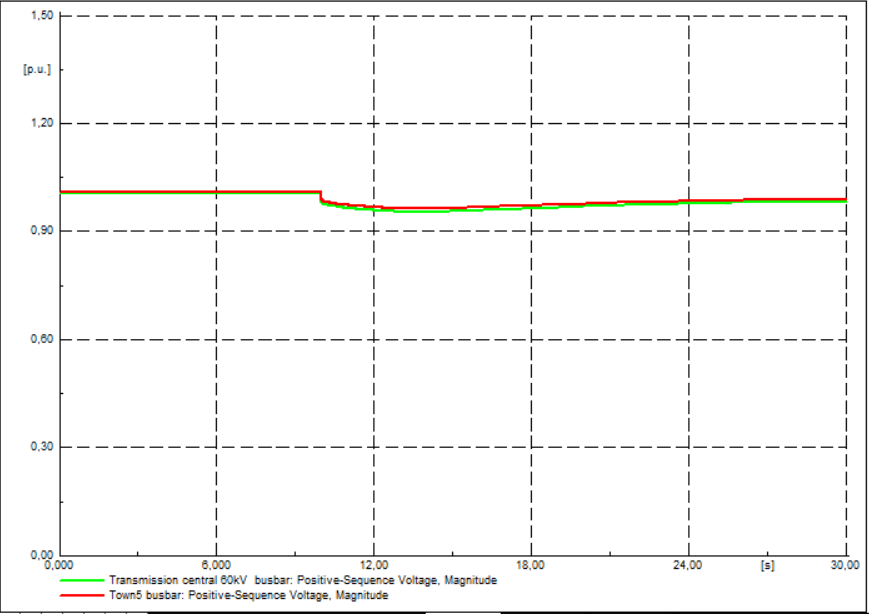
\includegraphics[width=1.00\textwidth]{figurer/LargeDisturbance/Voltage4} % Venstre billede
	\end{minipage}
	\hfill
	\begin{minipage}[b]{0.48\textwidth}
		\centering
		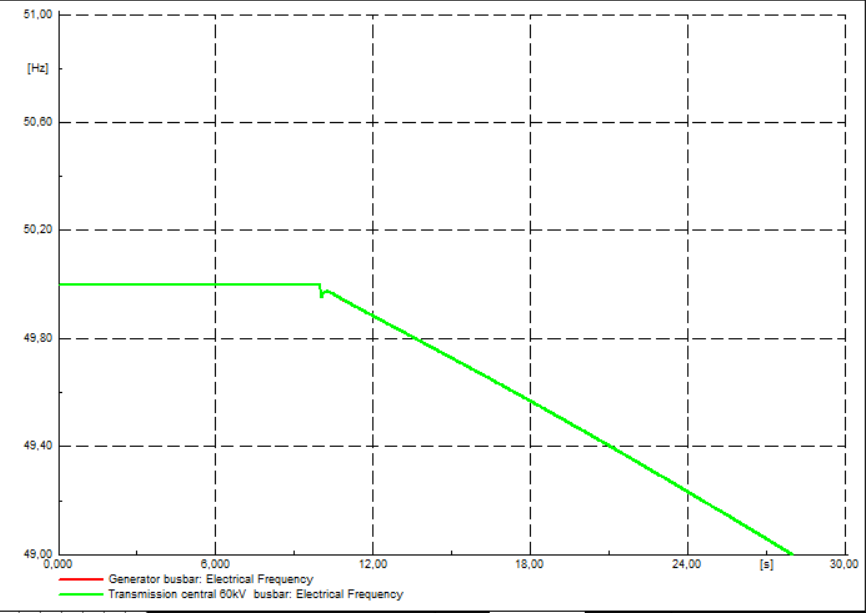
\includegraphics[width=1.00\textwidth]{figurer/LargeDisturbance/Freq4} % Højre billede
	\end{minipage}
	\\ % Figurtekster og labels
	\begin{minipage}[t]{0.48\textwidth}
		\caption{Case 2, Tilstand 4, Spændingsgraf} % Venstre figurtekst og label
		\label{fig:C2T4V}
	\end{minipage}
	\hfill
	\begin{minipage}[t]{0.48\textwidth}
		\caption{Case 2, Tilstand 4, Frekvensgraf} % Højre figurtekst og label
		\label{fig:C2T4F}
	\end{minipage}
\end{figure}

\begin{figure}[H] % (alternativt [H])
	\centering
	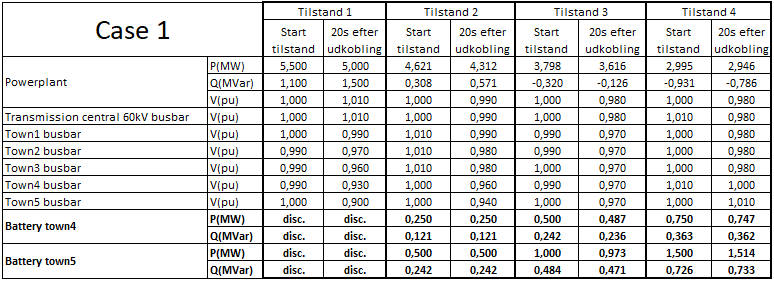
\includegraphics[width=1\textwidth]{figurer/SmallDisturbance/Overview}
	\caption{Overblik for spænding og effektoverførelse i nettet}
	\label{fig:C3Overview}
\end{figure}

Der observeres at når produktionen fra vindmølleparken udkobles vil der opleves et spændingsfald på både Town5 busbar - Town5 busbar er repræsentativ for alle byer - og Transmission central 60kV busbar. Det ses at spændingsfaldet i per unit er af samme størrelsesorden for både Town5 busbar og Transmission central 60kV busbar. På spændingsgraferne ses det at en stor andel af effektbidrag fra batteri vil resultere i et mindre spændingsfald ved udkobling. I tilstand 4, hvor byerne er selvforsynende, jf. \ref{fig:C3Overview}



I de 3 første tilstande observeres et spændingsfald ved Town5 busbar, når linjen 10kV Cable Town5 udkobles. Størrelsen afhænger af batteriernes effektbidrag. I tilstand 4 ses det at spændingen ved Town5 busbar stiger ved udkoblingen. Spænding ved Transmissions central 60kV busbar forbliver konstant på ca. 1pu i alle tilstande. Spændingsfaldet i tilstandende 1 - 3 er forventet, fordi tabet af den redundante linje vil øge kilde impedansen set fra Town5 busbar. Spændingsfaldet bliver mindre desto mere batteri effektbidrag pga. den reduceret strøm i transmissions og distributions kabler. Spændingsstigningen i tilstand 4 kan forklares ved at Town5 har større produktion end forbrug, derved vil den levere effekt til resten af systemet. Ved tab af 10kV Cable Town5, bliver load impedansen set fra Town5 busbar større og der vil opleves en spændingsstigning ved byens POC.

I de 4 tilstande ses det at frekvensen bliver mere stabilt ved større batteri bidrag. Stigningen på frekvensen i de første tilstande sker fordi at den samlede belastning bliver mindre da spændingen falder, produktionen forsøger at nedregulere, men kan ikke regulere hurtigt nok ift. belastningen. Dette sker ikke i tilstand 4 da spændingen ikke falder.